\documentclass[11pt]{article}
\usepackage{listings}
\usepackage{graphicx}
\usepackage{caption}
\usepackage{hyperref}
\def\subsectionautorefname{section}
\title{CMPUT 481 Assignment 1}
\author{Brock Toews}
\date{\today}
\begin{document}
\maketitle
\begin{center}
btoews

1284088
\end{center}
\thispagestyle{empty}
\pagebreak
\setcounter{page}{1}
\listoffigures
\tableofcontents
\pagebreak
\section{Introduction}
The purpose of this paper is to analyze the speedups gained by parallelizing a
simple widely spread algorithm: that of dense matrix multiplication. As one
will be able to see from what follows, the potential speedup of using multiple
CPU cores is quite great.
\section{Implementation}
\subsection{Description}
My sequential implementation is a simple, standard matrix multiplier. It was
written in C, and performs the following steps. First, it allocates three
single dimensional arrays: the two origin arrays, and the product array (this
step is shown as the \emph{Initalize} step in Figure \ref{fig:segment}). Then,
it walks through the two origin arrays, assigning random long integers to each
index (the \emph{Generate} step in Figure \ref{fig:segment}). Now, it walks
through both the origin arrays multiplying the proper indices together, storing
the results in an array of its own. Once an array has been completed, it sums
it together the array and assigns the result to the proper index of the product
array. This is the \emph{Multiply} step in Figure \ref{fig:segment}.

The parallelized version is a fairly intuitive adaptation of the above
implementation. Its initialization step is the same as the sequential
version's, except for one added component; it also generates a list of structs
storing the beginning and end of segments, where each of these segments are
computed by one thread. The generation step is performed in the same manner,
except that each segment is operated upon by a separate thread. After the
generation operations are complete, the threads are closed. And, just like
the generation step, the multiplication step is broken up into threads and
closed upon completion, with each thread operating upon one segment each.
\subsection{Correctness}
The correctness of the values generated by both implementation have not been
experimentally verified, as this is not exceedingly important to the
experiment. Instead, it has been checked that both implementations perform the
correct number of operations. It is also fairly certain that the resultant
values must be correct, from much reading of the code.
\subsection{Performance Considerations}
There are a few points regarding performance of the implementation that are
worth looking at. Firstly, one will immediately notice that between the
generation and multiplication steps, I close and reopen all of the threads,
while better performance could certainly be had by eliminated this sequential
part of the code. there are a couple reasons that this was not done. One, it is
somewhat easier to time the phases as a whole by returning to the main
function. Secondly, It as something of an arbitrary decision, as it seemed
easier to write at the time.

Another place where performance is in question is whether I make the program
cooperate with the machine's cache. In answer to this, yes. The nested
for-loops are functionally equivalent to looping through the single dimensional
arrays with one loop, without making any large jumps. As such, most of the
matrix accesses should be cache hits.
\section{Analysis of Results}
\subsection{Dataset Decisions}
It is, of course, quite necessary to establish what kind of data was used in
the execution of the experiment. There were three sizes of matrix that were
considered: 1024x1024, 2048x2048, and 4096x4096. Each of these sizes were run
in the sequential version, and in the parallel version with 2 through 8
threads. Finally, for each set of parameters, the test was run 10 times,
throwing out the first 5.

It should be noted that 512x512 tests were also run, but the results were not
considered for various reasons. While the results were interesting and unique
from the other tests, they were thrown out for various reasons, among those
reasons, the small amount of time it took to run the tests (and the inherent
unreliablility of short times), and the simple fact that it was inconvenient to
make the charts easily readable when there was the one set of data with values
so tiny.

Finally, the hardware that the tests were run on is important. For the
experiment, I used a laptop with an Intel Core i7 running 4 (hyperthreaded)
cores.
\subsection{Performance Gains}
Now, after much adeiu, we may discuss the numbers of the experiment. The first
item of significance, is the speedup (Figure \ref{fig:speedup}). once can see up to
four cores, one almost gets linear speedup. This, on its own, very much
demonstrates the advantage of parallelization.

An interesting note of this that one will definitely notice, is that after four
threads (5-8), the speedup levels off. This is quite likely a result of the
i7's use of hyperthreading to create logical threads.\\

Unsuprisingly, as one can see in Figure \ref{fig:segment}, most time of the
computation is spent in the multiplication stage. This stage take less and less
time as more cores are added.

What is more suprising, is that the generation phase takes more time as more
cores are added. What the reason for this is, is unclear. It is not a
sequential section, nor is the amount of work there is to do dependent on the
number of threads. The only reasoning that comes to mind is that the compiler
has an easier time optimizing the, admittedly, simple generation code when it
is sequential.
\section{Conclusion}
As one can see from Figures \ref{fig:speedup} and \ref{fig:time}, and above
discussion, using multiple threads to perform easily parallelizable operations
provides a significant performance advantage over simply running the same code
sequentially, in a single thread.
\begin{figure}
\centering
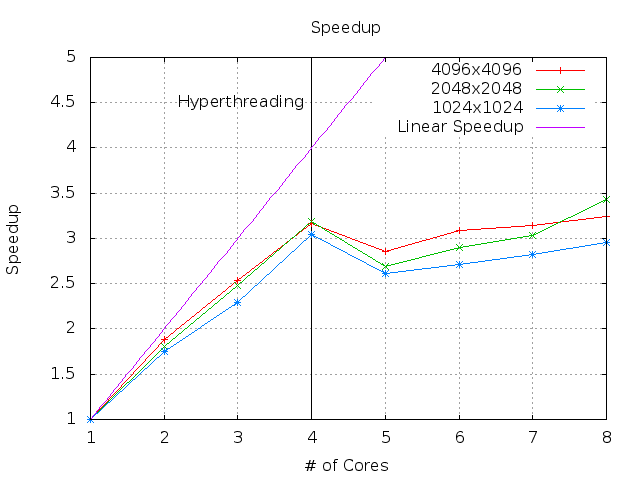
\includegraphics[width=300pt]{speedup.png}
\caption{Chart of speedups}
\label{fig:speedup}
\end{figure}
\begin{figure}
\centering
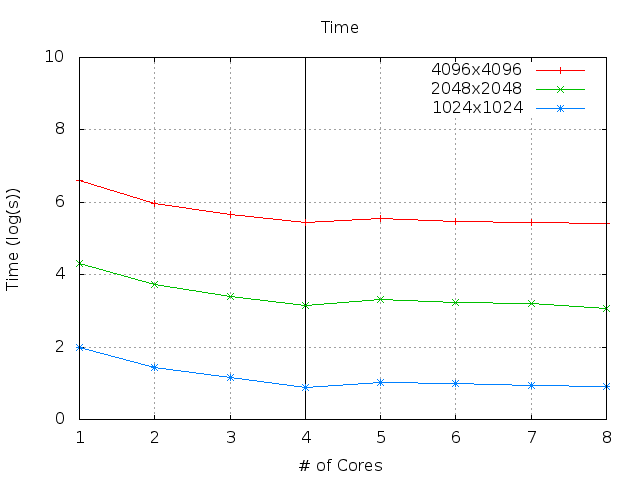
\includegraphics[width=300pt]{time.png}
\caption{Chart of times to multiply matrices}
\label{fig:time}
\end{figure}
\begin{figure}
\centering
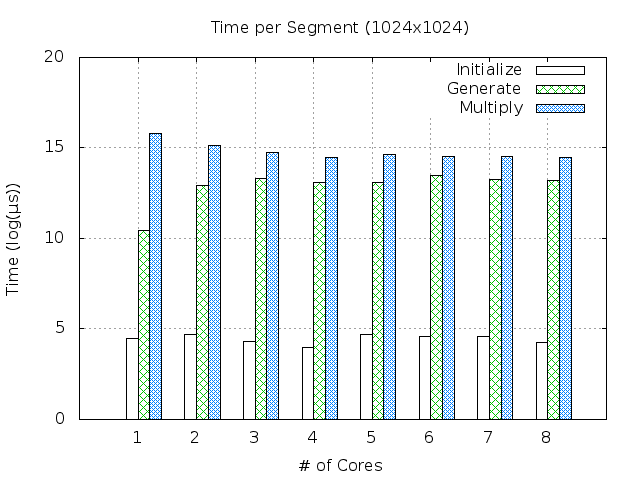
\includegraphics[width=300pt]{segment.png}
\caption{Chart of times to complete segments}
\label{fig:segment}
\end{figure}
\pagebreak
\section{Source Code}
\lstset{numbers=left, language=C}
\subsection{Parallel Implementation}
\lstinputlisting{main.c}
\pagebreak
\subsection{Sequential Implementation}
\lstinputlisting{seq.c}
\subsection{Analysis Script}
\lstinputlisting[language=Python]{average.py}
\subsection{Gnuplot Script}
\lstinputlisting{plot}
\subsection{Makefile}
\lstinputlisting{Makefile}
\subsection{Raw Data}
\lstinputlisting{output.dat}
\lstinputlisting{average.dat}
\end{document}
